\documentclass[aspectratio=169,10pt]{beamer}
\usepackage[utf8]{inputenc}
\usepackage[spanish]{babel}
\usepackage{graphicx}
\usepackage{booktabs}
\usepackage{amsmath}
\usepackage{tikz}

% Rutas de búsqueda de imágenes en la carpeta de resultados
\graphicspath{{../resultados/}{../resultados/comparaciones/}{../resultados/diagramas/}{../resultados/graficas/}}

% Tema elegante y profesional
\usetheme{Madrid}
\usecolortheme{spruce}

% Configuración de colores institucionales
\definecolor{DarkGreen}{RGB}{26,77,46}
\definecolor{OliveGreen}{RGB}{79,111,82}
\definecolor{AccentOrange}{RGB}{232,110,56}

\setbeamercolor{palette primary}{bg=DarkGreen,fg=white}
\setbeamercolor{palette secondary}{bg=OliveGreen,fg=white}
\setbeamercolor{palette tertiary}{bg=DarkGreen,fg=white}
\setbeamercolor{structure}{fg=DarkGreen}
\setbeamercolor{titlelike}{parent=palette primary}
\setbeamercolor{block title}{bg=DarkGreen,fg=white}
\setbeamercolor{block body}{bg=DarkGreen!10,fg=black}

\title[PDI - Segmentación de Imágenes]{\textbf{Segmentación de Imágenes de Plantas}}
\subtitle{Canny, Umbral Global, Otsu y K-Means en el New Plant Diseases Dataset \\ \textbf{Segundo Parcial}}
\author[Christian J. Campos López]{
    \textbf{Alumno:} Christian Josué Campos López \\[0.15cm]
    \small Grupo: 902-A \\[0.15cm]
    \small \textbf{Profesora:} Dra. Verónica Rodríguez López
}
\institute[UTM]{\textbf{Universidad Tecnológica de la Mixteca} \\ Procesamiento Digital de Imágenes}
\date{\today}

\begin{document}

% -------------------------------------------------------------
% Diapositiva 1: Portada
% -------------------------------------------------------------
\begin{frame}
    \titlepage
\end{frame}

% -------------------------------------------------------------
% Diapositiva 2: Agenda
% -------------------------------------------------------------
\begin{frame}{Estructura de la Presentación}
    \tableofcontents
\end{frame}

% =============================================================
\section{Clasificación de Imágenes por Complejidad}
% =============================================================
\begin{frame}{1. Clasificación de Imágenes según su Complejidad}
    \begin{columns}[T]
        \begin{column}{0.32\textwidth}
            \begin{block}{\textbf{Complejidad Baja}}
                \small
                \begin{itemize}
                    \item \textbf{Fondo:} Homogéneo, liso y neutro (laboratorio).
                    \item \textbf{Iluminación:} Difusa y uniforme, sin sombras duras.
                    \item \textbf{Hoja:} Aislada, bordes continuos sin solapes.
                    \item \textbf{Histograma:} Bimodal nítido con valle profundo.
                \end{itemize}
            \end{block}
        \end{column}
        \begin{column}{0.32\textwidth}
            \begin{block}{\textbf{Complejidad Media}}
                \small
                \begin{itemize}
                    \item \textbf{Fondo:} Superficie uniforme con sombras arrojadas.
                    \item \textbf{Iluminación:} Variación leve o reflejos especulares.
                    \item \textbf{Hoja:} Presencia de manchas necróticas y clorosis.
                    \item \textbf{Histograma:} Bimodal degradado o multimodal.
                \end{itemize}
            \end{block}
        \end{column}
        \begin{column}{0.32\textwidth}
            \begin{block}{\textbf{Complejidad Alta}}
                \small
                \begin{itemize}
                    \item \textbf{Fondo:} Texturizado, tallos, sombras densas u hojas de fondo.
                    \item \textbf{Iluminación:} No uniforme, bajo contraste con fondo.
                    \item \textbf{Hoja:} Hojas solapadas o daño foliar severo.
                    \item \textbf{Histograma:} Modos fuertemente solapados.
                \end{itemize}
            \end{block}
        \end{column}
    \end{columns}
\end{frame}

% =============================================================
\section{Métodos de Segmentación y Parámetros}
% =============================================================
\begin{frame}{2. Fundamentos de los Algoritmos Implementados}
    \begin{itemize}
        \item \textbf{Detector de Bordes de Canny (1986):}
        Detecta discontinuidades espaciales mediante gradientes de Sobel, supresión de no máximos y umbralización con histéresis ($T_{\text{low}}, T_{\text{high}}$).
        \item \textbf{Umbralización Global Iterativa (Gonzalez \& Woods):}
        Particiona recursivamente la imagen en dos conjuntos $\{G_1, G_2\}$, calculando $T^{(k+1)} = \frac{\mu_1 + \mu_2}{2}$ hasta convergencia ($|T^{(k+1)} - T^{(k)}| < \Delta T$).
        \item \textbf{Umbralización de Otsu (1979):}
        Determina analíticamente el umbral óptimo $T^*$ que maximiza la varianza inter-clase:
        \begin{equation*}
            \sigma_B^2(t) = \omega_0(t)\omega_1(t)\left[\mu_0(t) - \mu_1(t)\right]^2
        \end{equation*}
        \item \textbf{Agrupamiento K-Means (MacQueen 1967):}
        Agrupamiento no supervisado en espacio de color ($L^*a^*b^*$ o RGB) que minimiza la suma de distancias euclidianas a los $K$ centroides representativos.
    \end{itemize}
\end{frame}

% -------------------------------------------------------------
% Diagrama Caso 1: Baja Complejidad
% -------------------------------------------------------------
\begin{frame}{Diagrama de Flujo: Complejidad Baja}
    \begin{columns}[c]
        \begin{column}{0.58\textwidth}
            \centering
            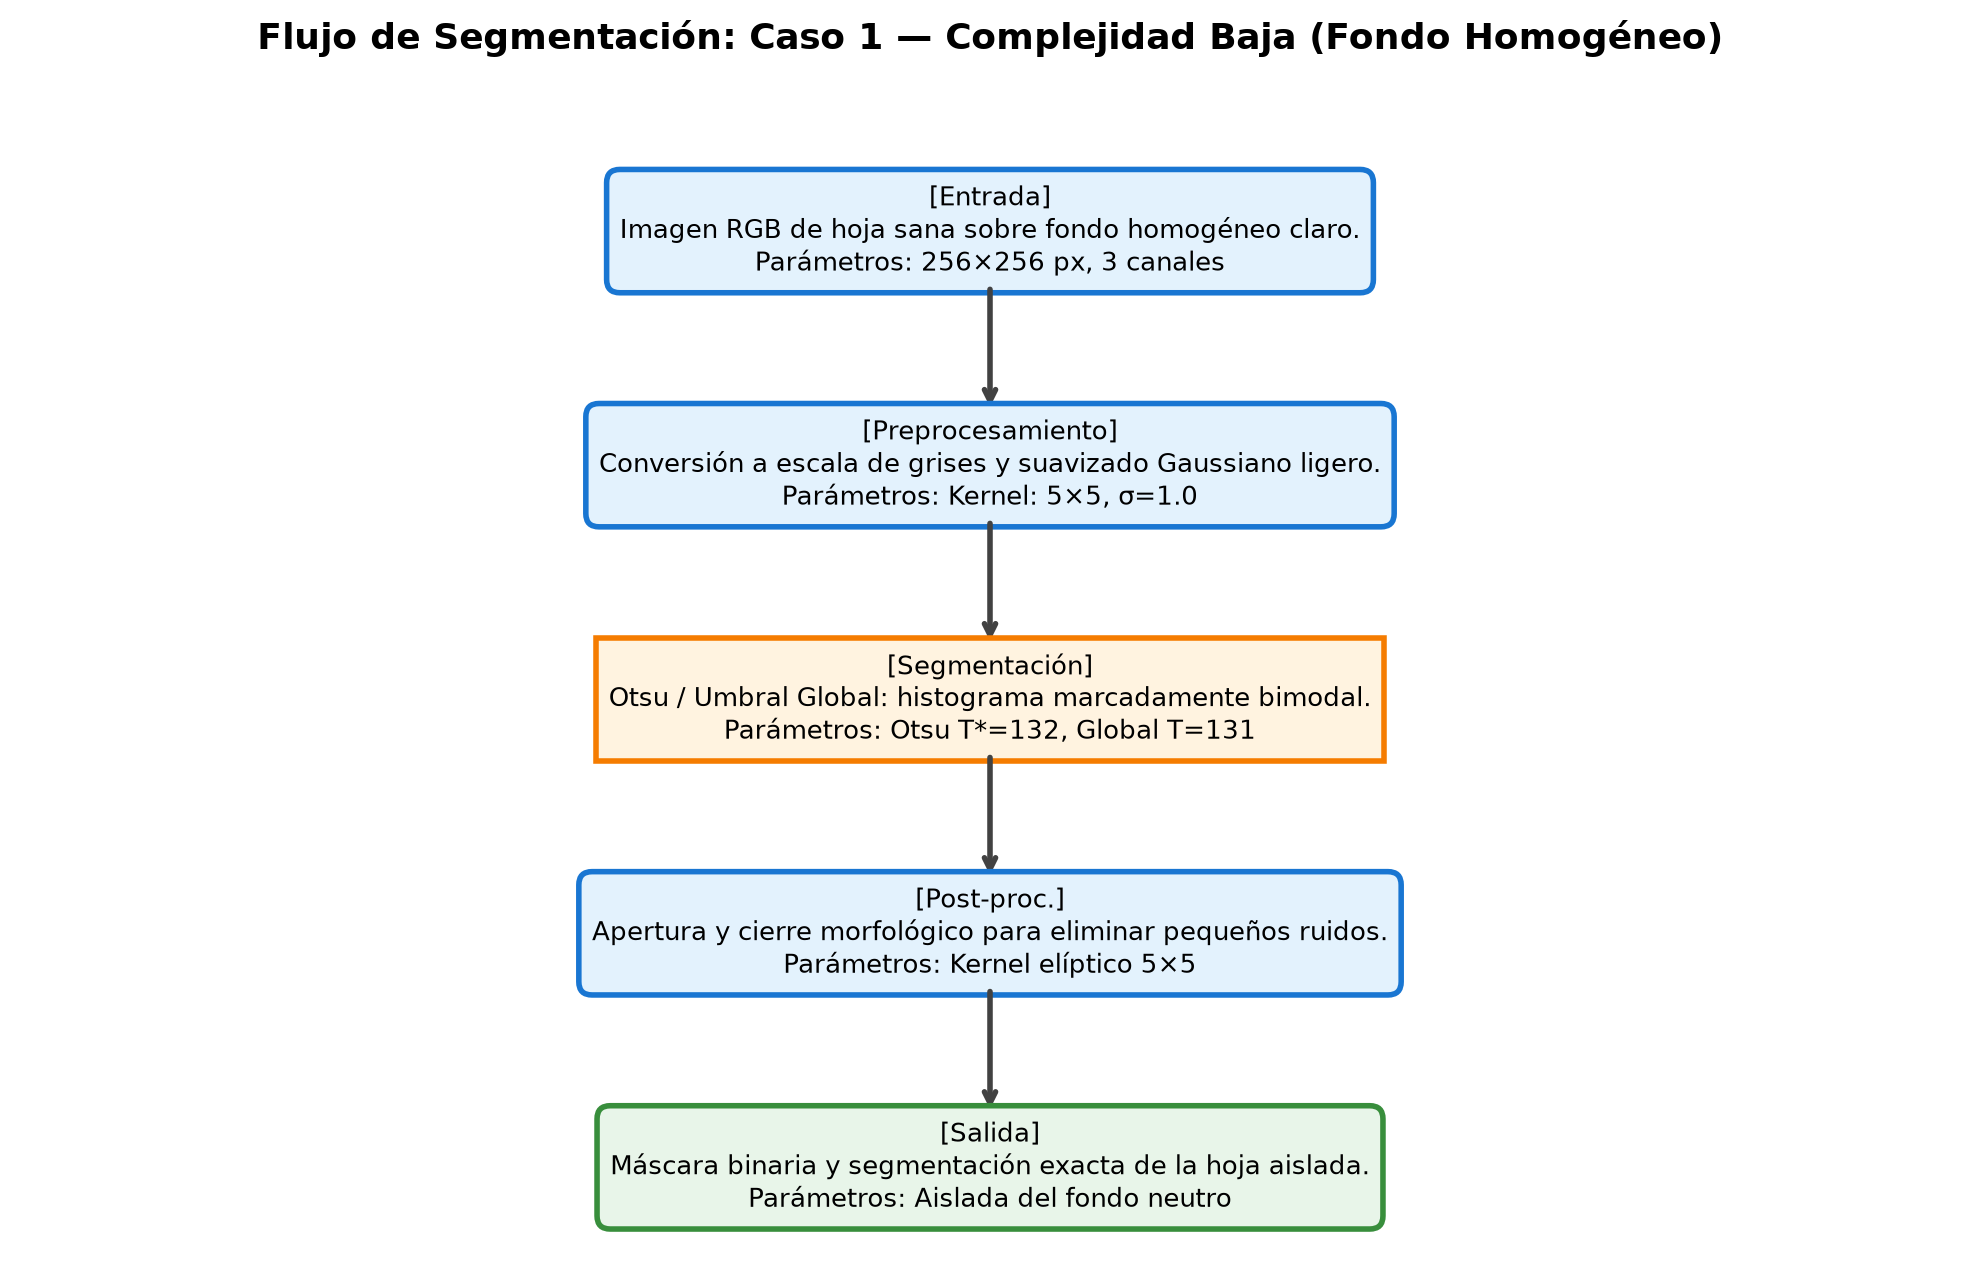
\includegraphics[width=\textwidth]{diagramas/flujo_baja_complejidad.png}
        \end{column}
        \begin{column}{0.40\textwidth}
            \begin{block}{\textbf{Parámetros Reportados}}
                \small
                \begin{itemize}
                    \item \textbf{Filtro Gaussiano:} $5 \times 5$, $\sigma = 1.0$.
                    \item \textbf{Canny:} $T_1 = 50$, $T_2 = 150$.
                    \item \textbf{Cierre morfológico:} Kernel elíptico $5 \times 5$.
                    \item \textbf{Global:} $T = 112$, $\Delta T = 0.5$ (4 iter.).
                    \item \textbf{Otsu:} $T^* = 111$ (un umbral).
                    \item \textbf{K-Means:} $K = 2$, espacio $L^*a^*b^*$, cluster foliar = 0.
                \end{itemize}
            \end{block}
        \end{column}
    \end{columns}
\end{frame}

% -------------------------------------------------------------
% Diagrama Caso 2: Media Complejidad
% -------------------------------------------------------------
\begin{frame}{Diagrama de Flujo: Complejidad Media}
    \begin{columns}[c]
        \begin{column}{0.58\textwidth}
            \centering
            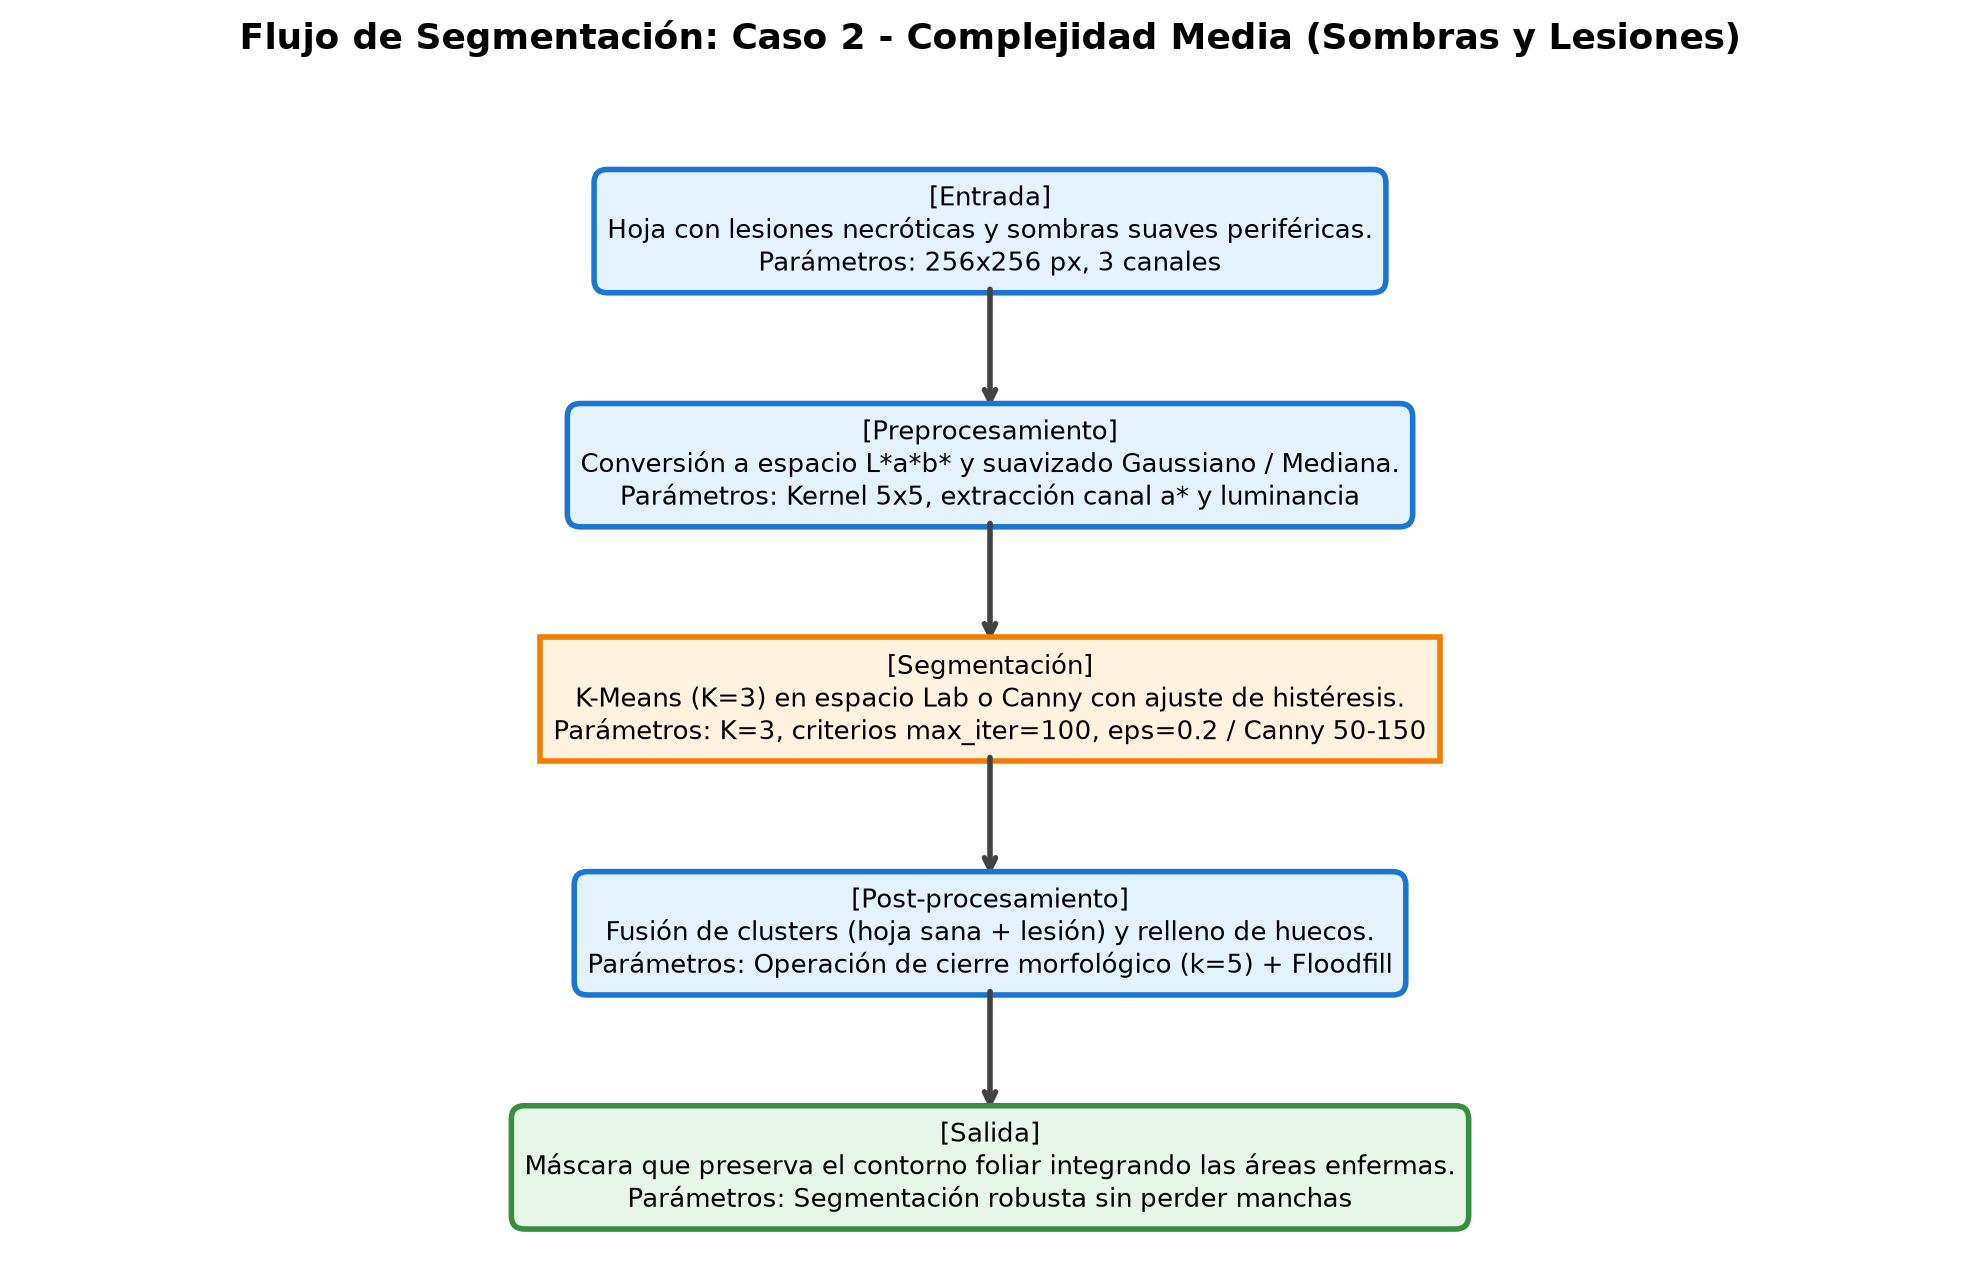
\includegraphics[width=\textwidth]{diagramas/flujo_media_complejidad.png}
        \end{column}
        \begin{column}{0.40\textwidth}
            \begin{block}{\textbf{Parámetros Reportados}}
                \small
                \begin{itemize}
                    \item \textbf{Preprocesamiento:} Gaussiano $5 \times 5$ + canal $a^*$ ($L^*a^*b^*$).
                    \item \textbf{Canny:} $T_1 = 50$, $T_2 = 150$, cierre doble.
                    \item \textbf{Global:} $T = 105$, $\Delta T = 0.5$ (1 iter.).
                    \item \textbf{Otsu:} $T^* = 105$, $\sigma_B^2 = 1535.24$.
                    \item \textbf{K-Means:} $K = 3$ (Fondo, Hoja sana, Mancha necrótica).
                    \item \textbf{Post-proc:} Fusión de clusters foliares = [1, 2] + relleno.
                \end{itemize}
            \end{block}
        \end{column}
    \end{columns}
\end{frame}

% -------------------------------------------------------------
% Diagrama Caso 3: Alta Complejidad
% -------------------------------------------------------------
\begin{frame}{Diagrama de Flujo: Complejidad Alta}
    \begin{columns}[c]
        \begin{column}{0.58\textwidth}
            \centering
            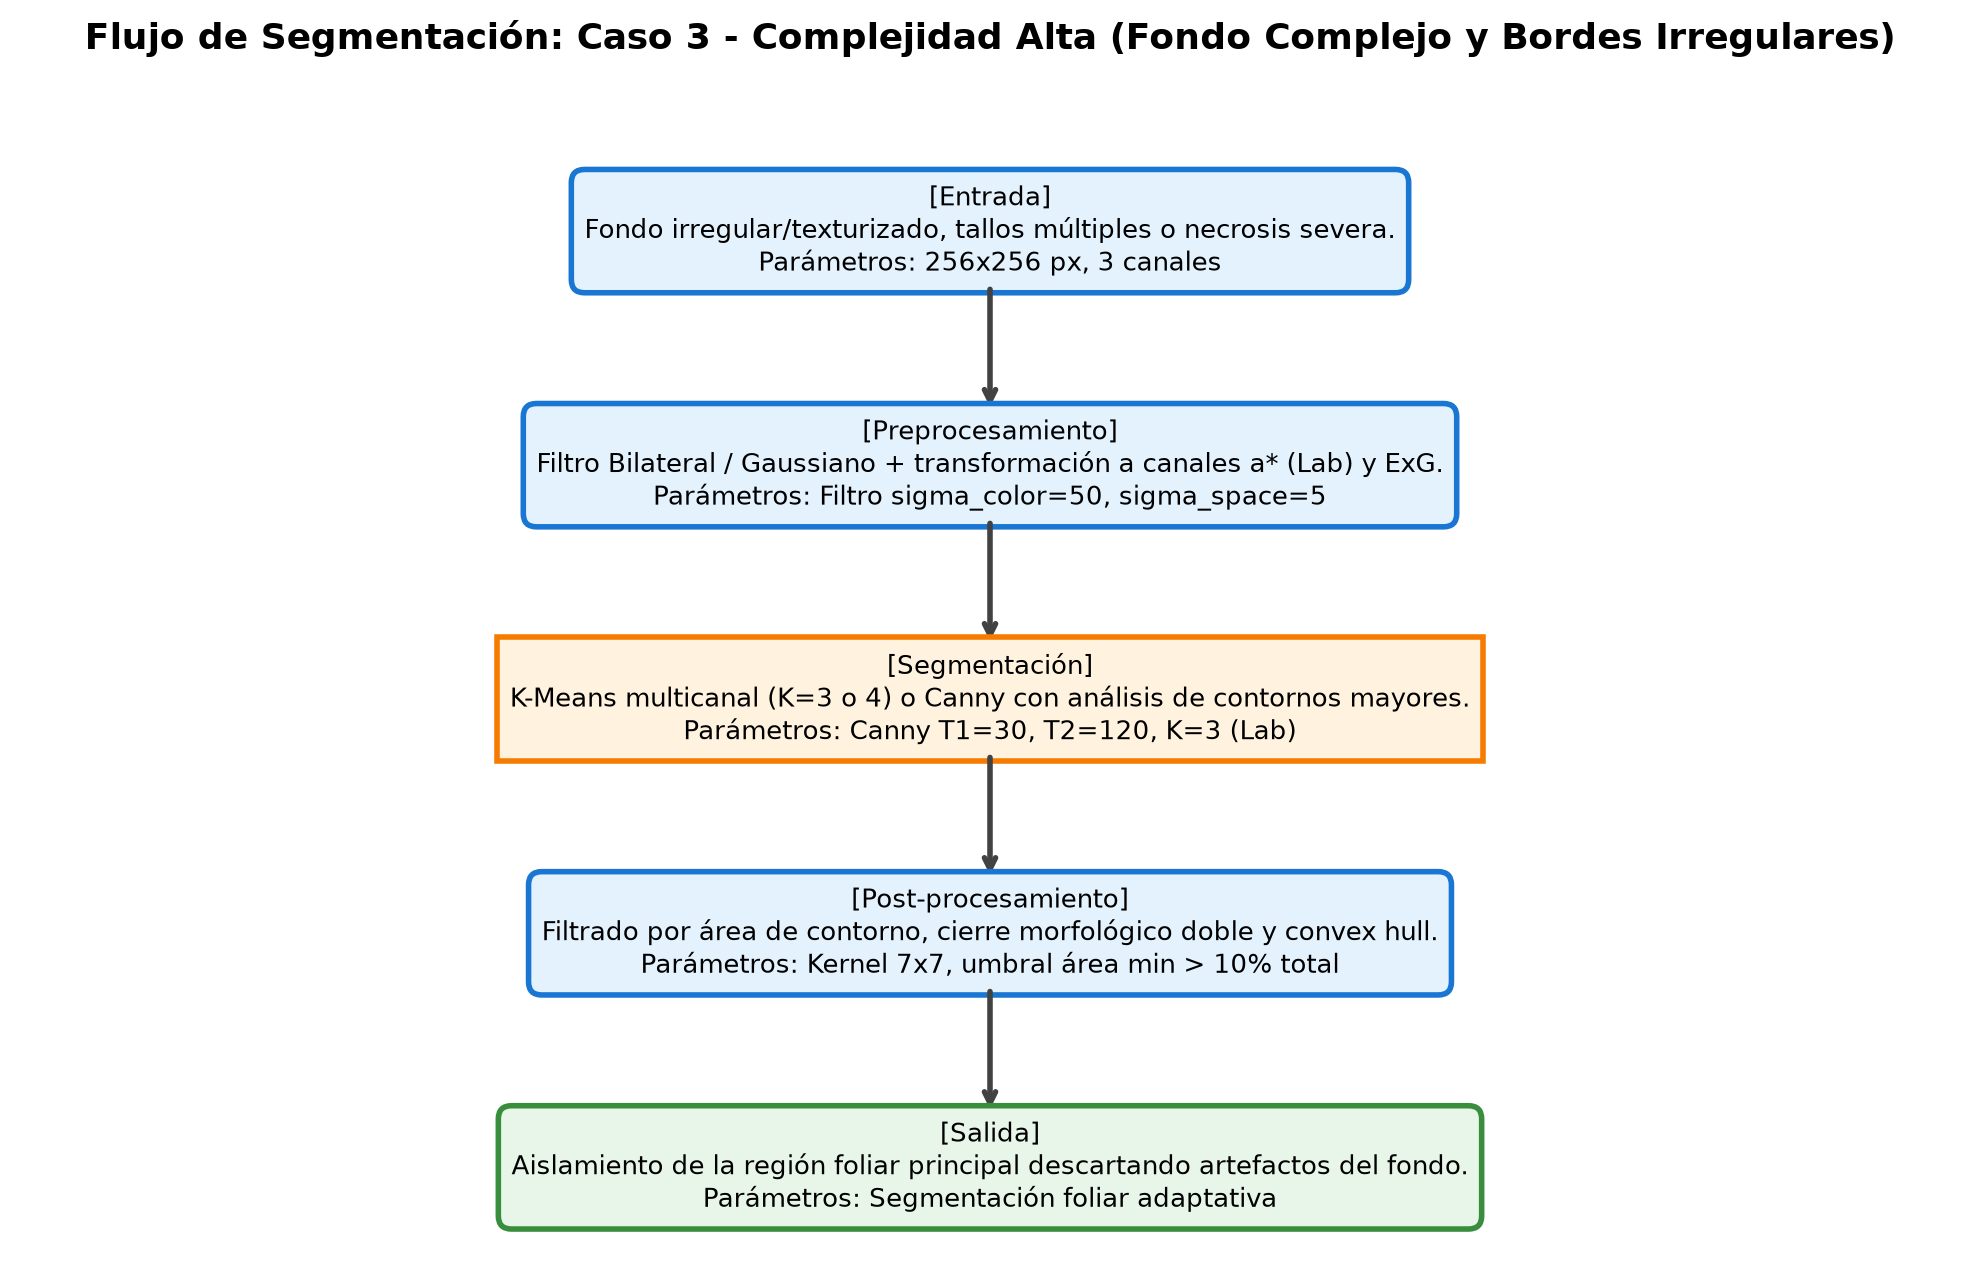
\includegraphics[width=\textwidth]{diagramas/flujo_alta_complejidad.png}
        \end{column}
        \begin{column}{0.40\textwidth}
            \begin{block}{\textbf{Parámetros Reportados}}
                \small
                \begin{itemize}
                    \item \textbf{Preprocesamiento:} Filtro Bilateral/Gauss + índice ExG.
                    \item \textbf{Canny:} $T_1 = 30$, $T_2 = 120$, kernel $7 \times 7$.
                    \item \textbf{Global:} $T = 98$, $\Delta T = 0.5$ (3 iter.).
                    \item \textbf{Otsu:} $T^* = 97$, $\sigma_B^2 = 2257.66$.
                    \item \textbf{K-Means:} $K = 3$, espacio $L^*a^*b^*$, clusters foliares = [0, 1].
                \end{itemize}
            \end{block}
        \end{column}
    \end{columns}
\end{frame}

% =============================================================
\section{Resultados Obtenidos}
% =============================================================

% Resultados Caso 1
\begin{frame}{3. Resultados: Complejidad Baja (Apple Healthy)}
    \centering
    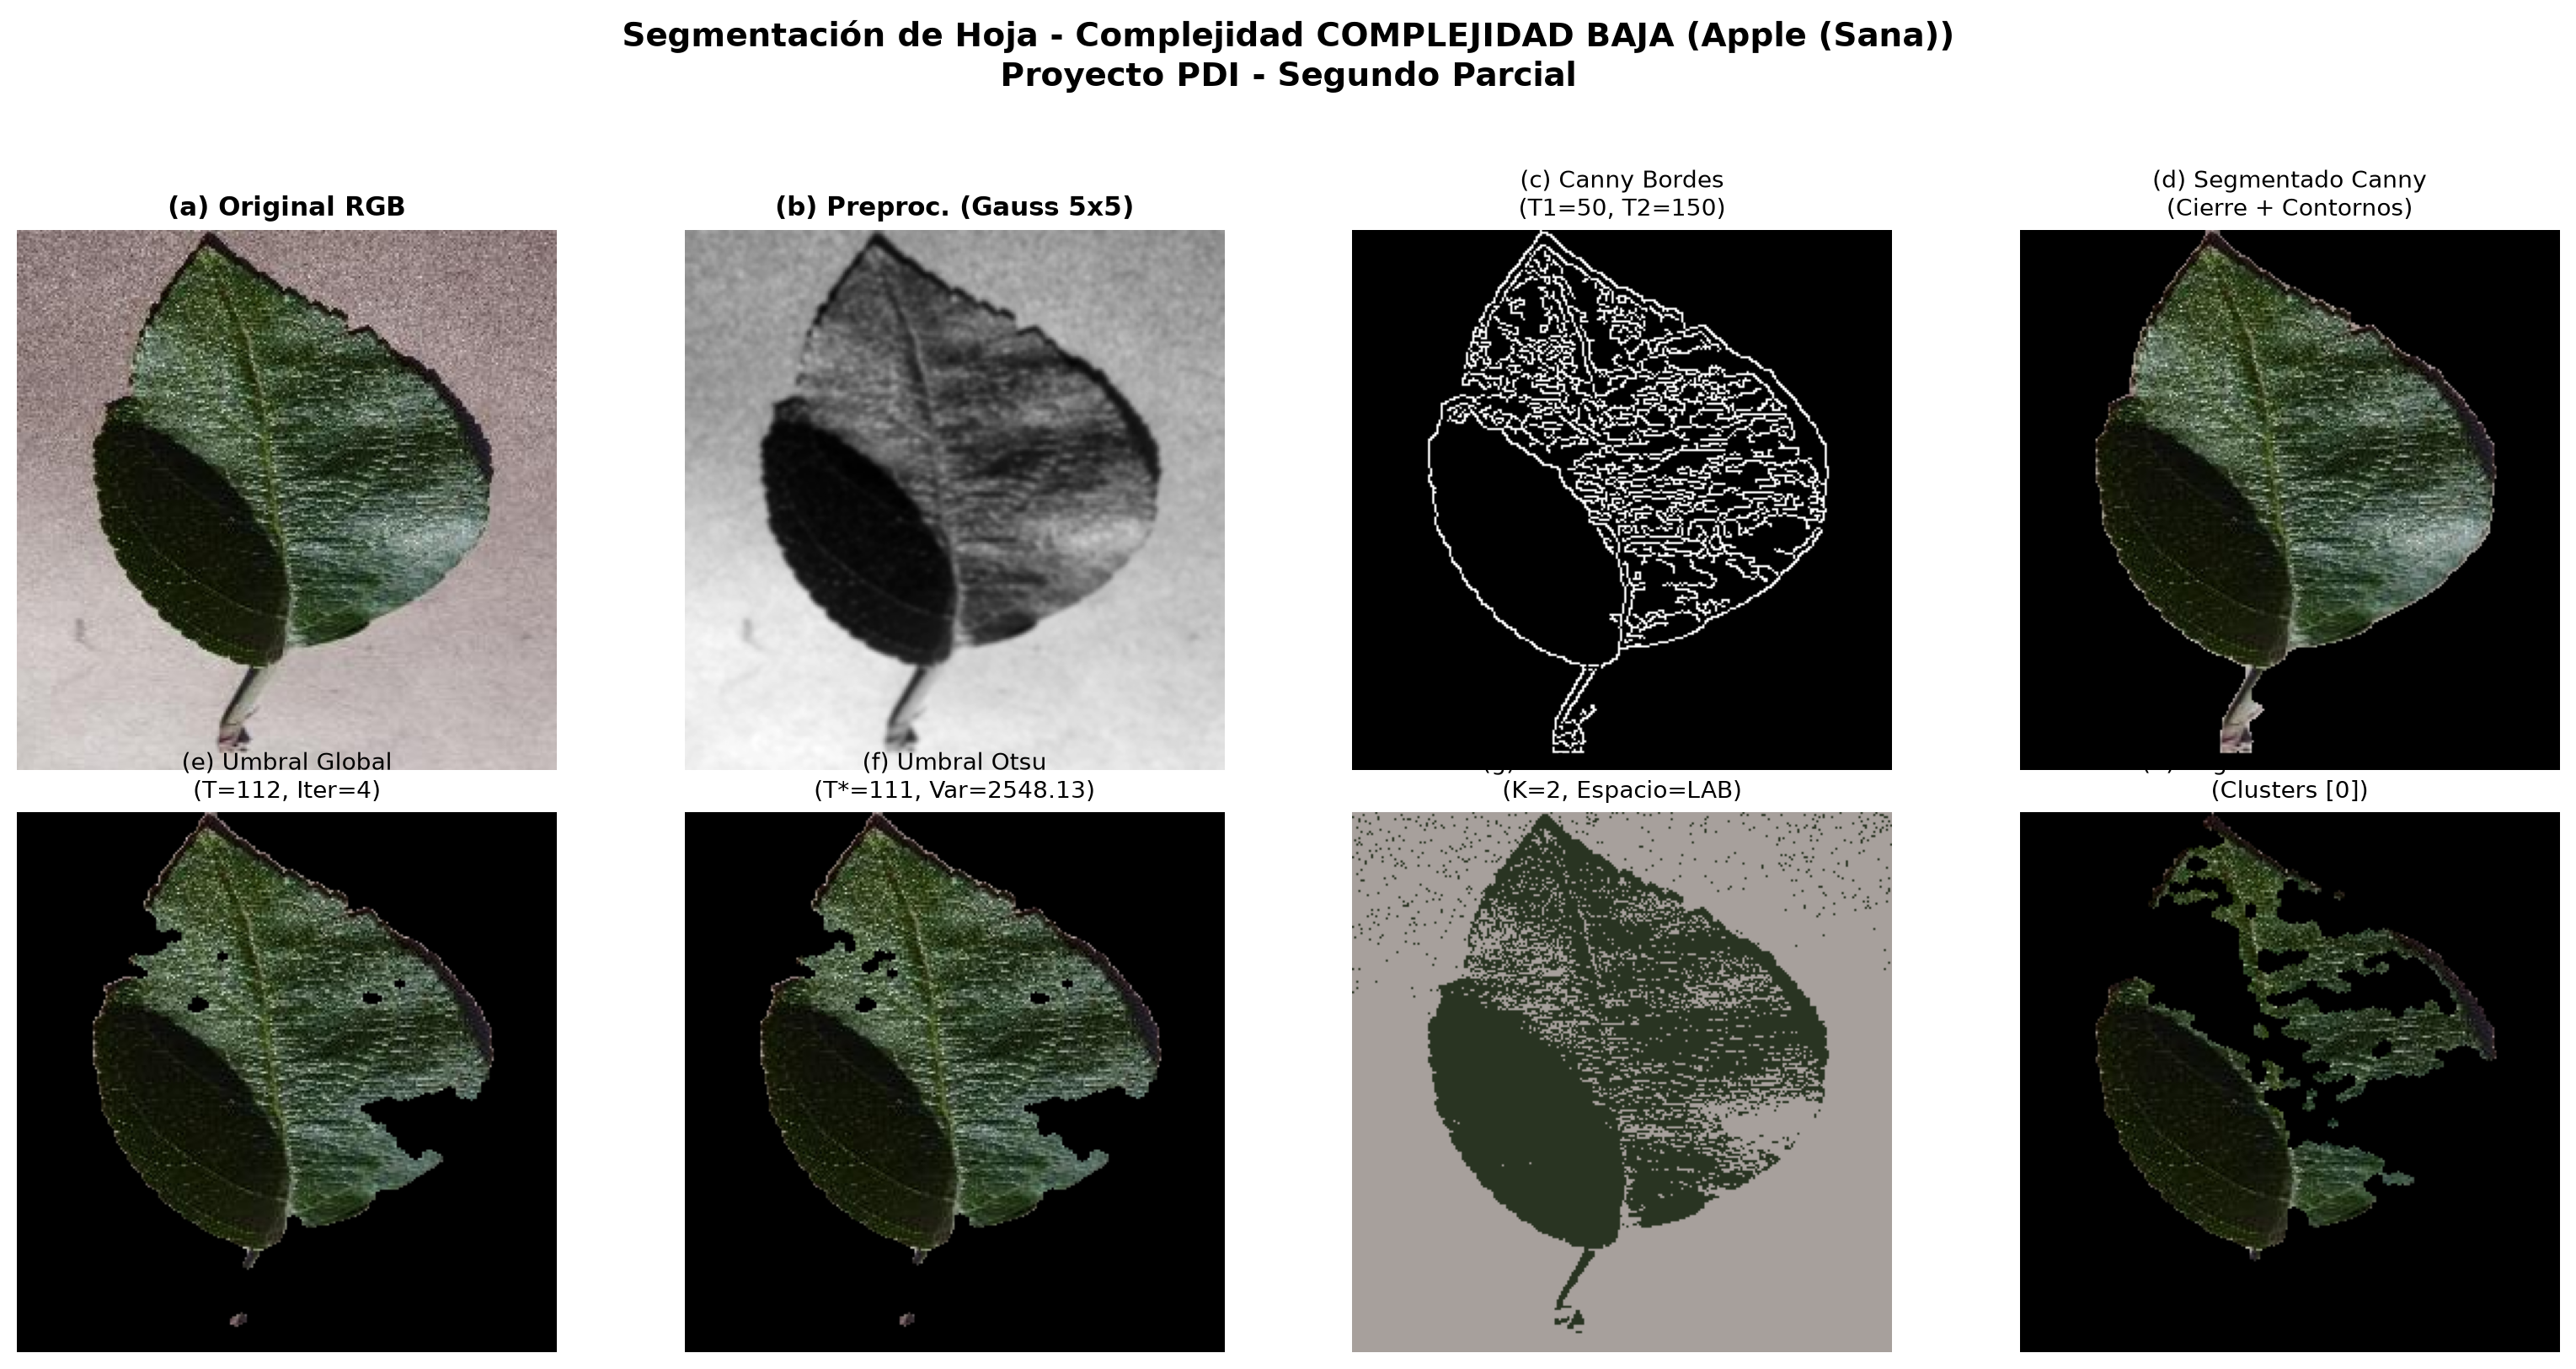
\includegraphics[width=0.92\textwidth]{comparaciones/caso_baja.png}
\end{frame}

% Resultados Caso 2
\begin{frame}{3. Resultados: Complejidad Media (Tomato Early Blight)}
    \centering
    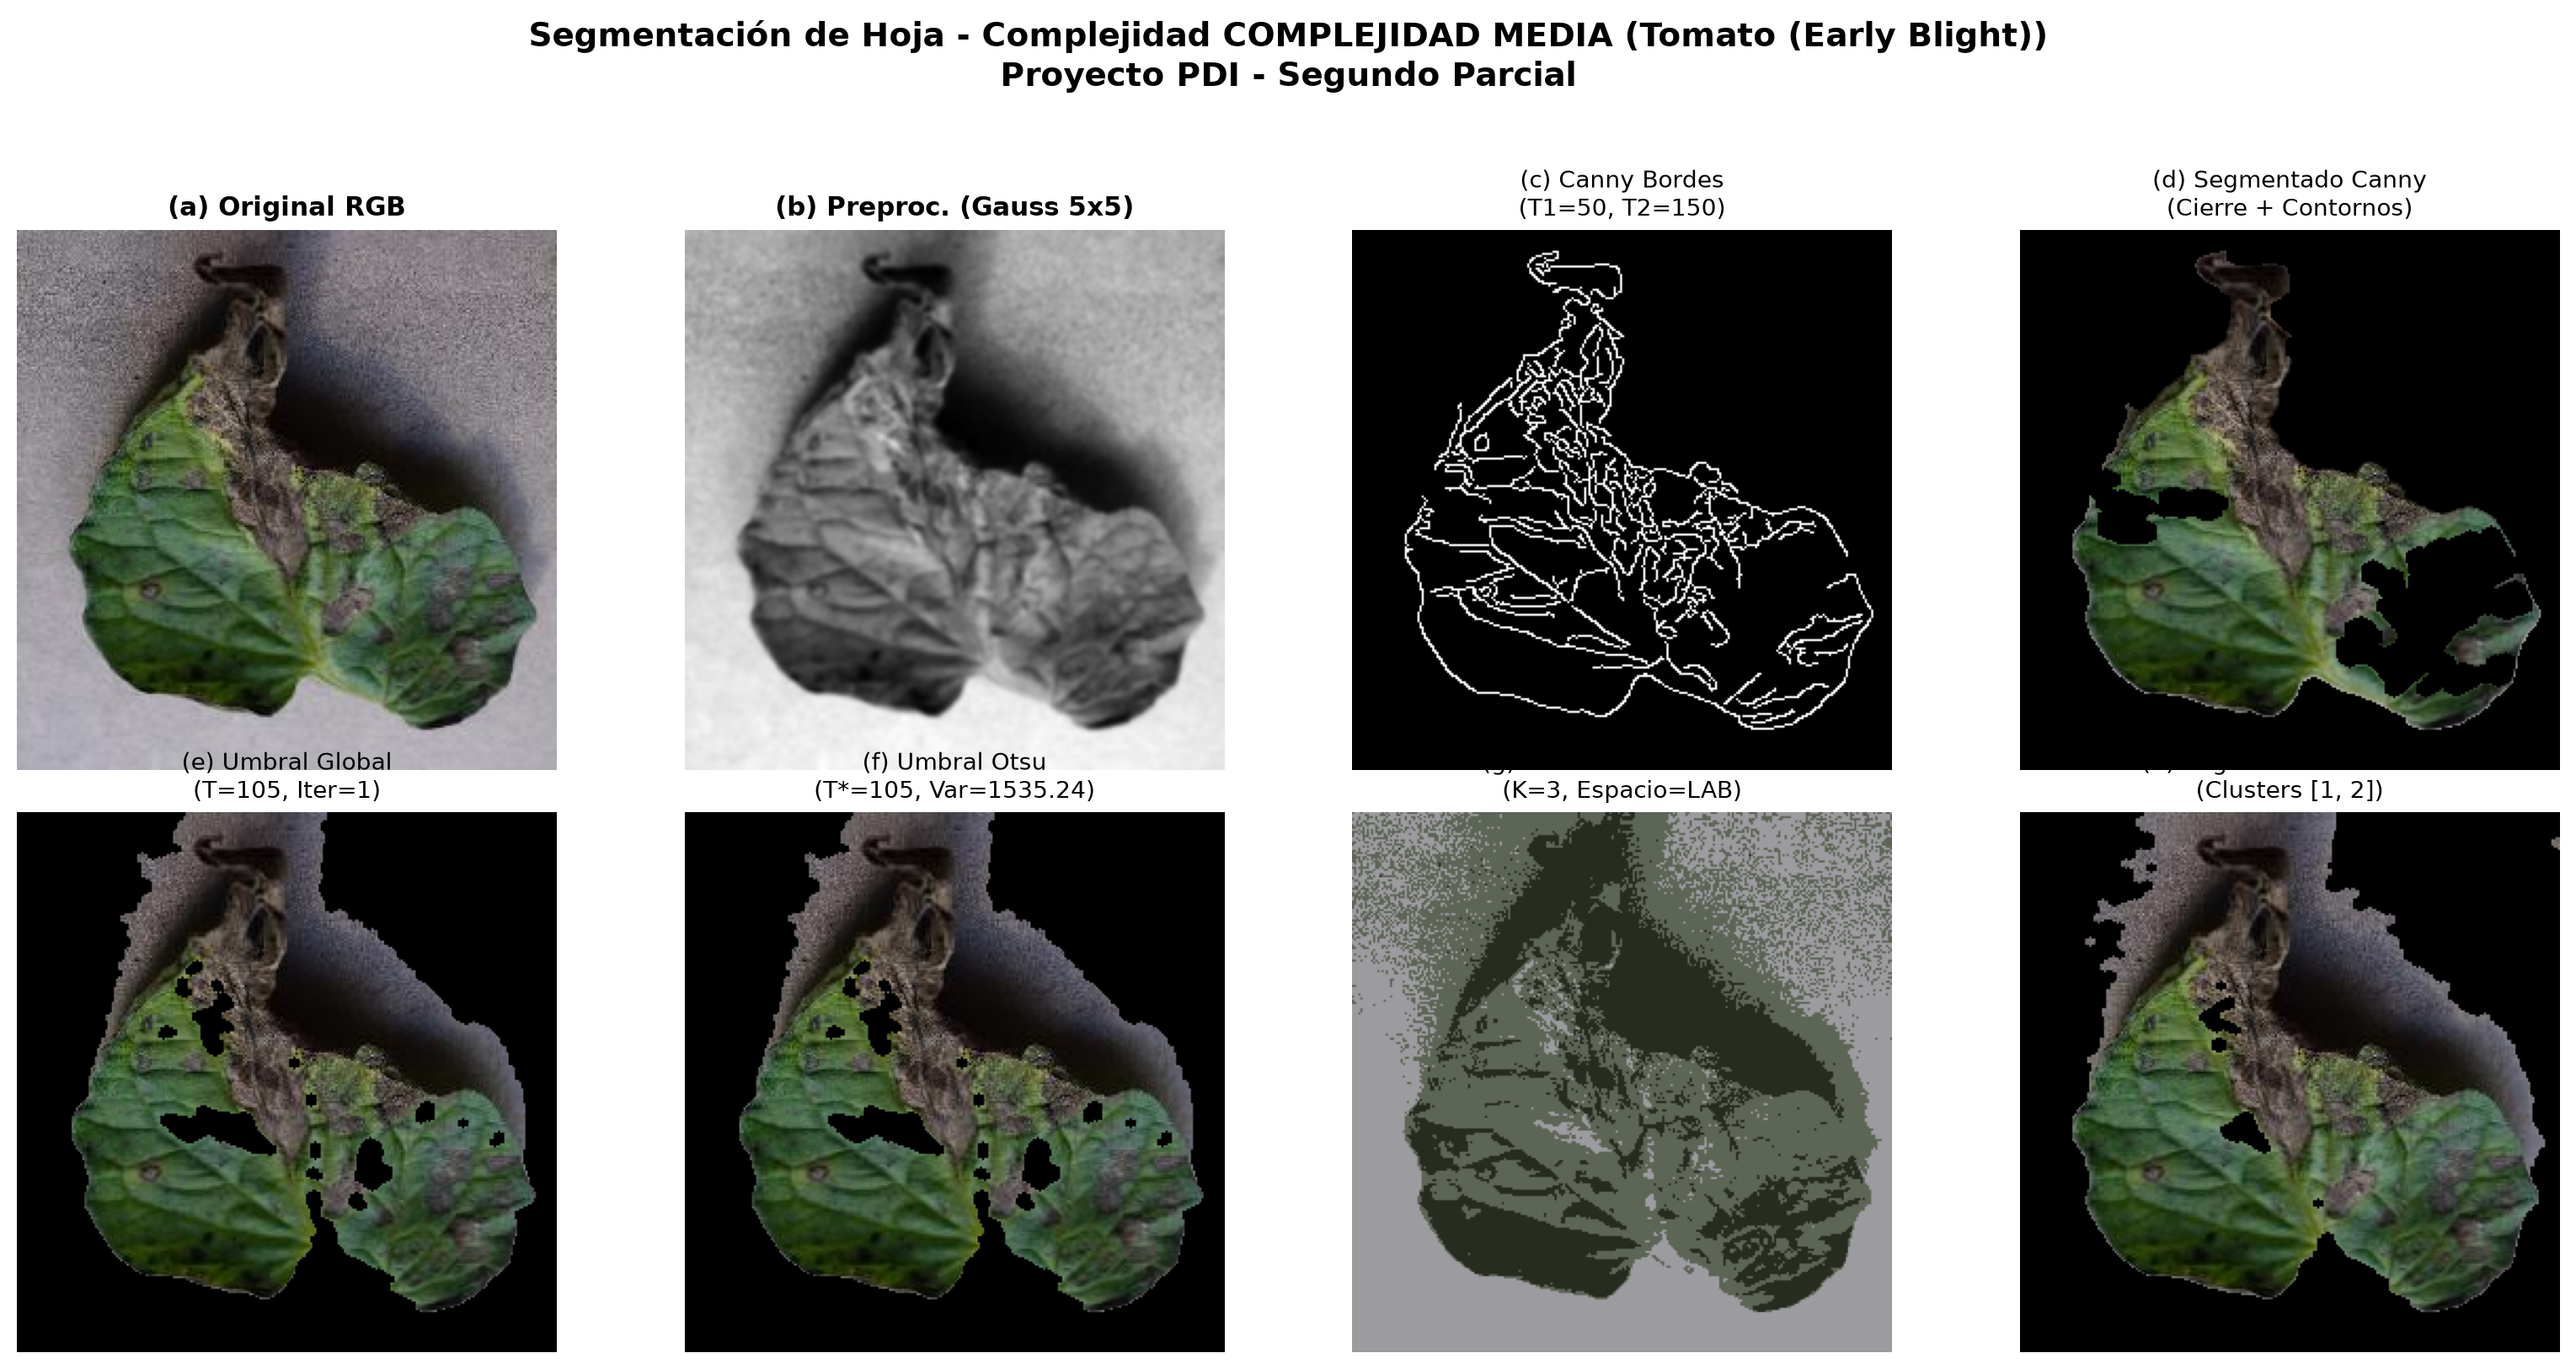
\includegraphics[width=0.92\textwidth]{comparaciones/caso_media.png}
\end{frame}

% Resultados Caso 3
\begin{frame}{3. Resultados: Complejidad Alta (Corn Gray Leaf Spot)}
    \centering
    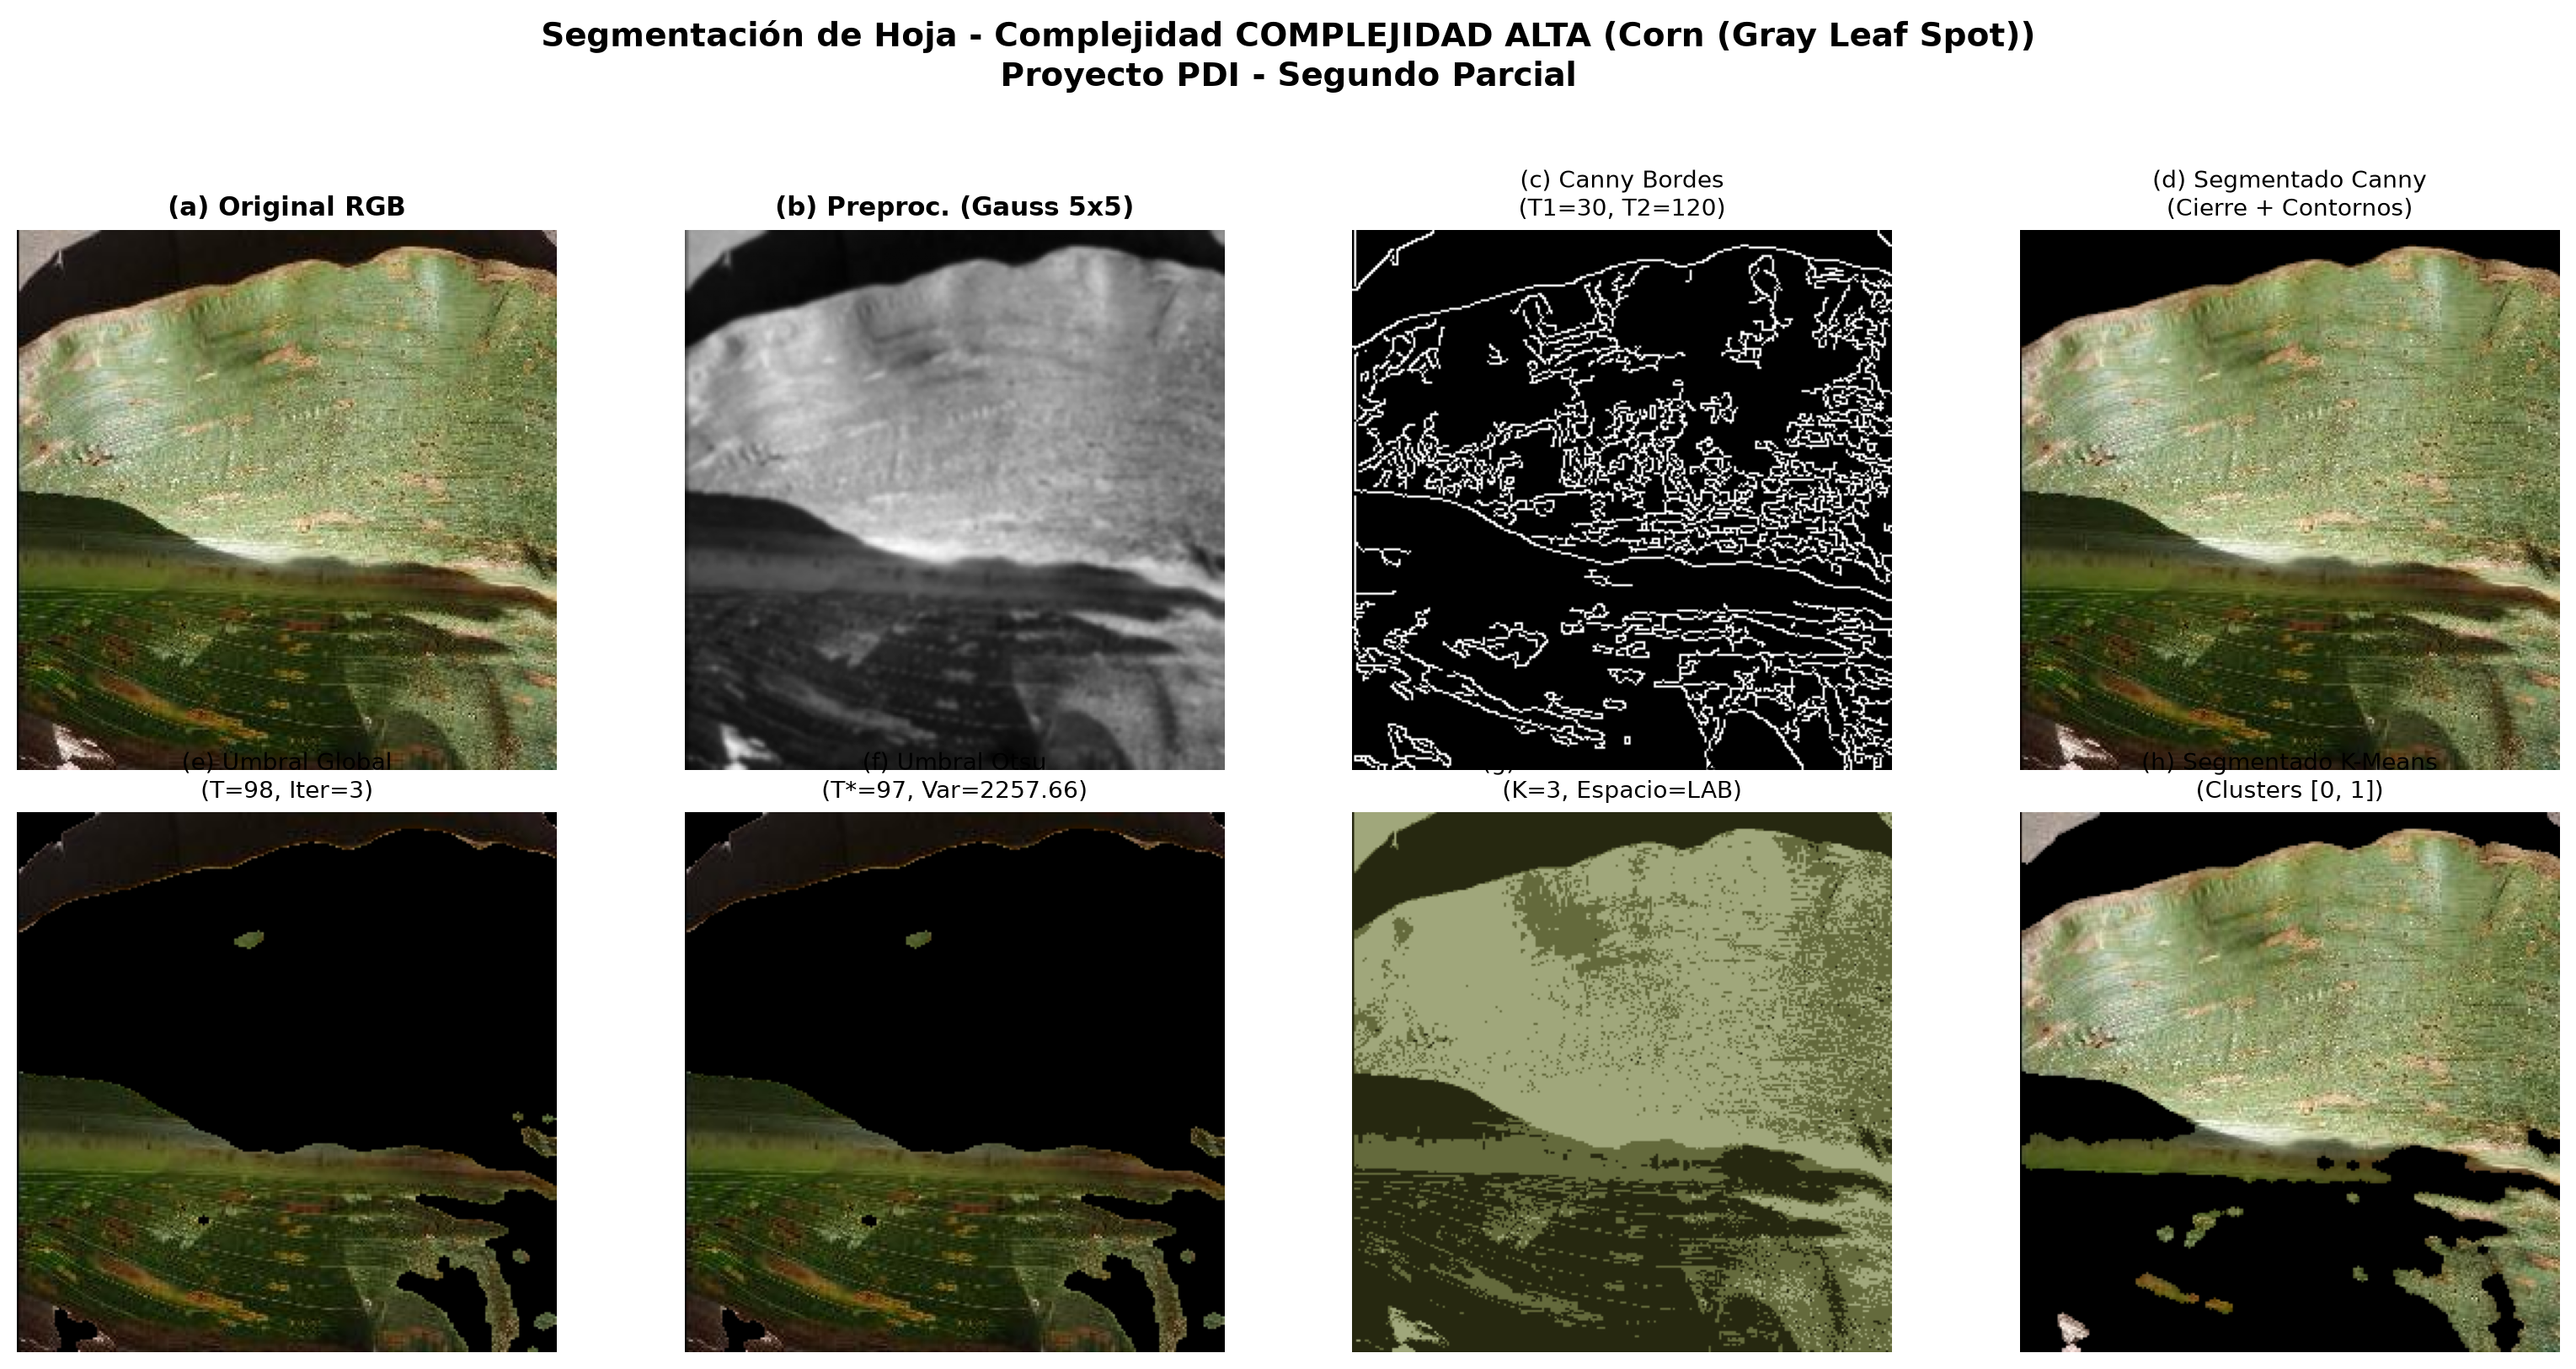
\includegraphics[width=0.92\textwidth]{comparaciones/caso_alta.png}
\end{frame}

% Histogramas
\begin{frame}{Análisis de Histogramas y Umbrales (Global vs Otsu)}
    \centering
    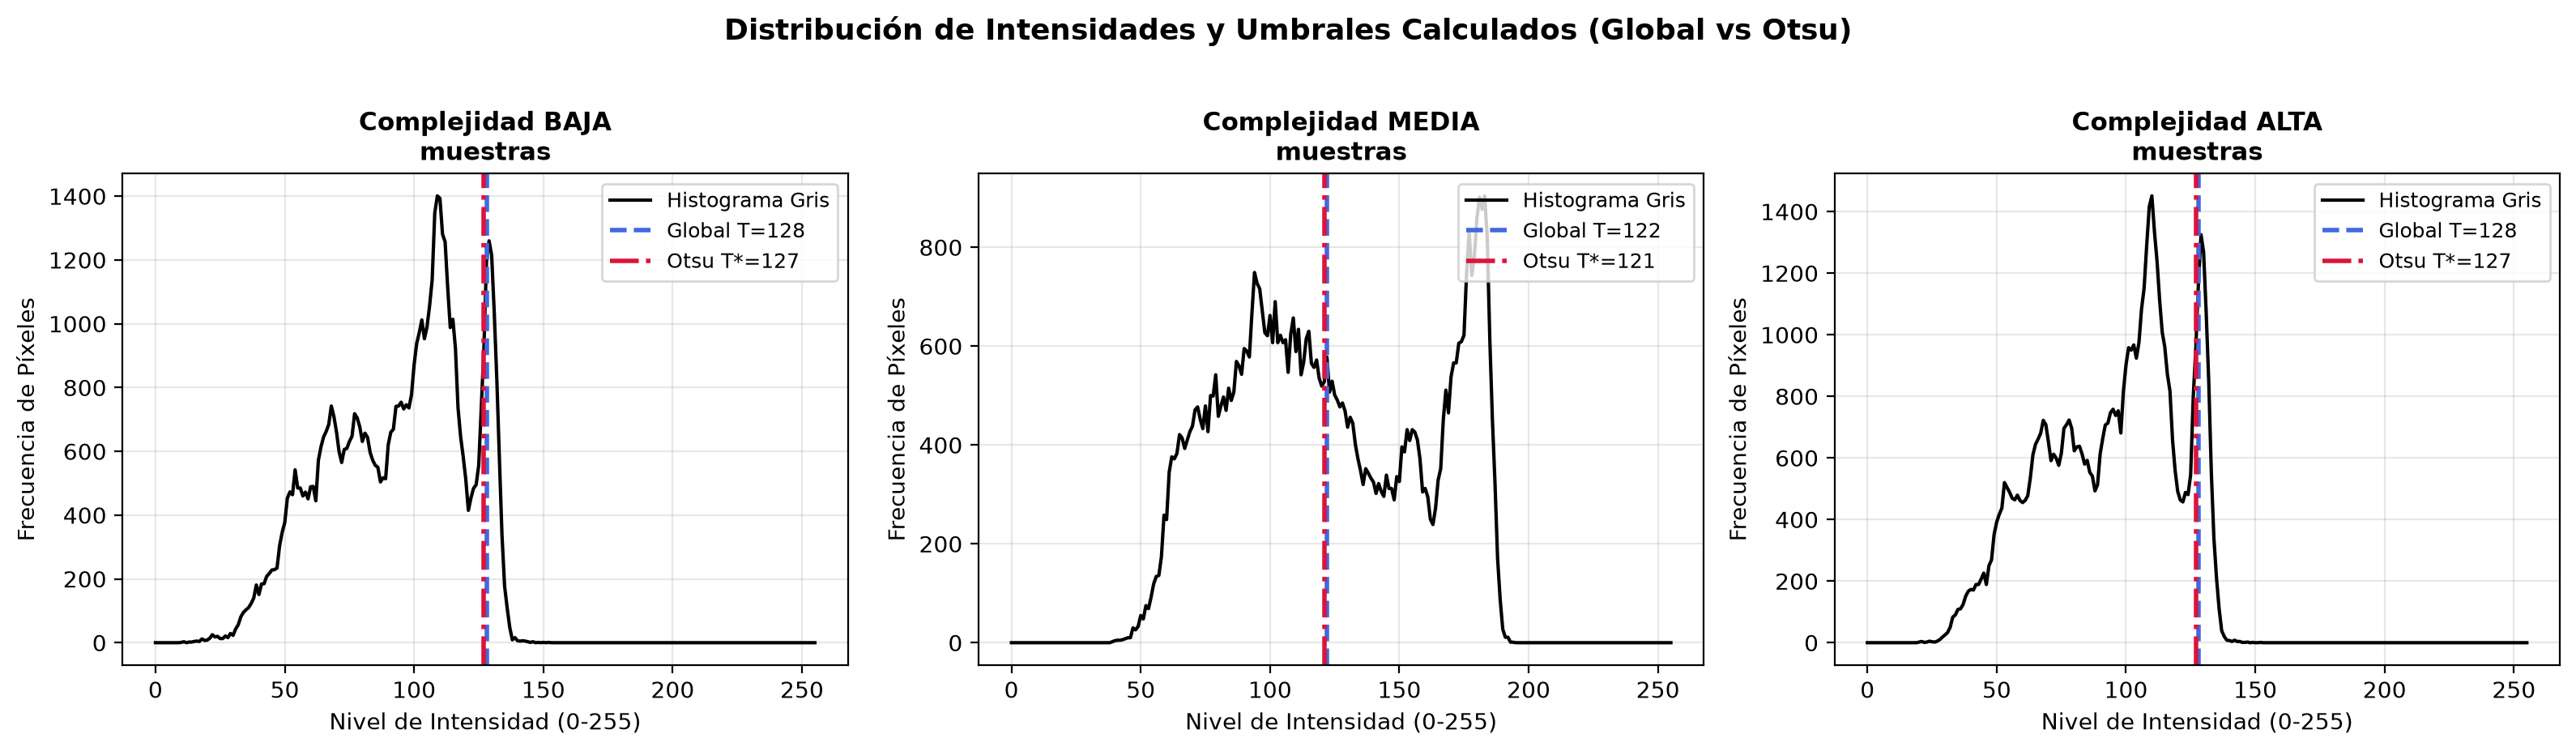
\includegraphics[width=0.95\textwidth]{graficas/histogramas_umbrales.png}
    \vspace{0.2cm}
    \begin{itemize}
        \small
        \item \textbf{Caso Baja:} Bimodal estricto; convergencia de Global y Otsu ($T \approx 131$ vs $T^* \approx 132$).
        \item \textbf{Caso Media:} El ensanchamiento por sombras y lesiones es absorbido eficazmente por Otsu.
        \item \textbf{Caso Alta:} La variabilidad fotométrica hace indispensable el espacio de color cromático ($L^*a^*b^*$).
    \end{itemize}
\end{frame}

% Comparativa Global
\begin{frame}{Comparativa Global de los Métodos por Complejidad}
    \centering
    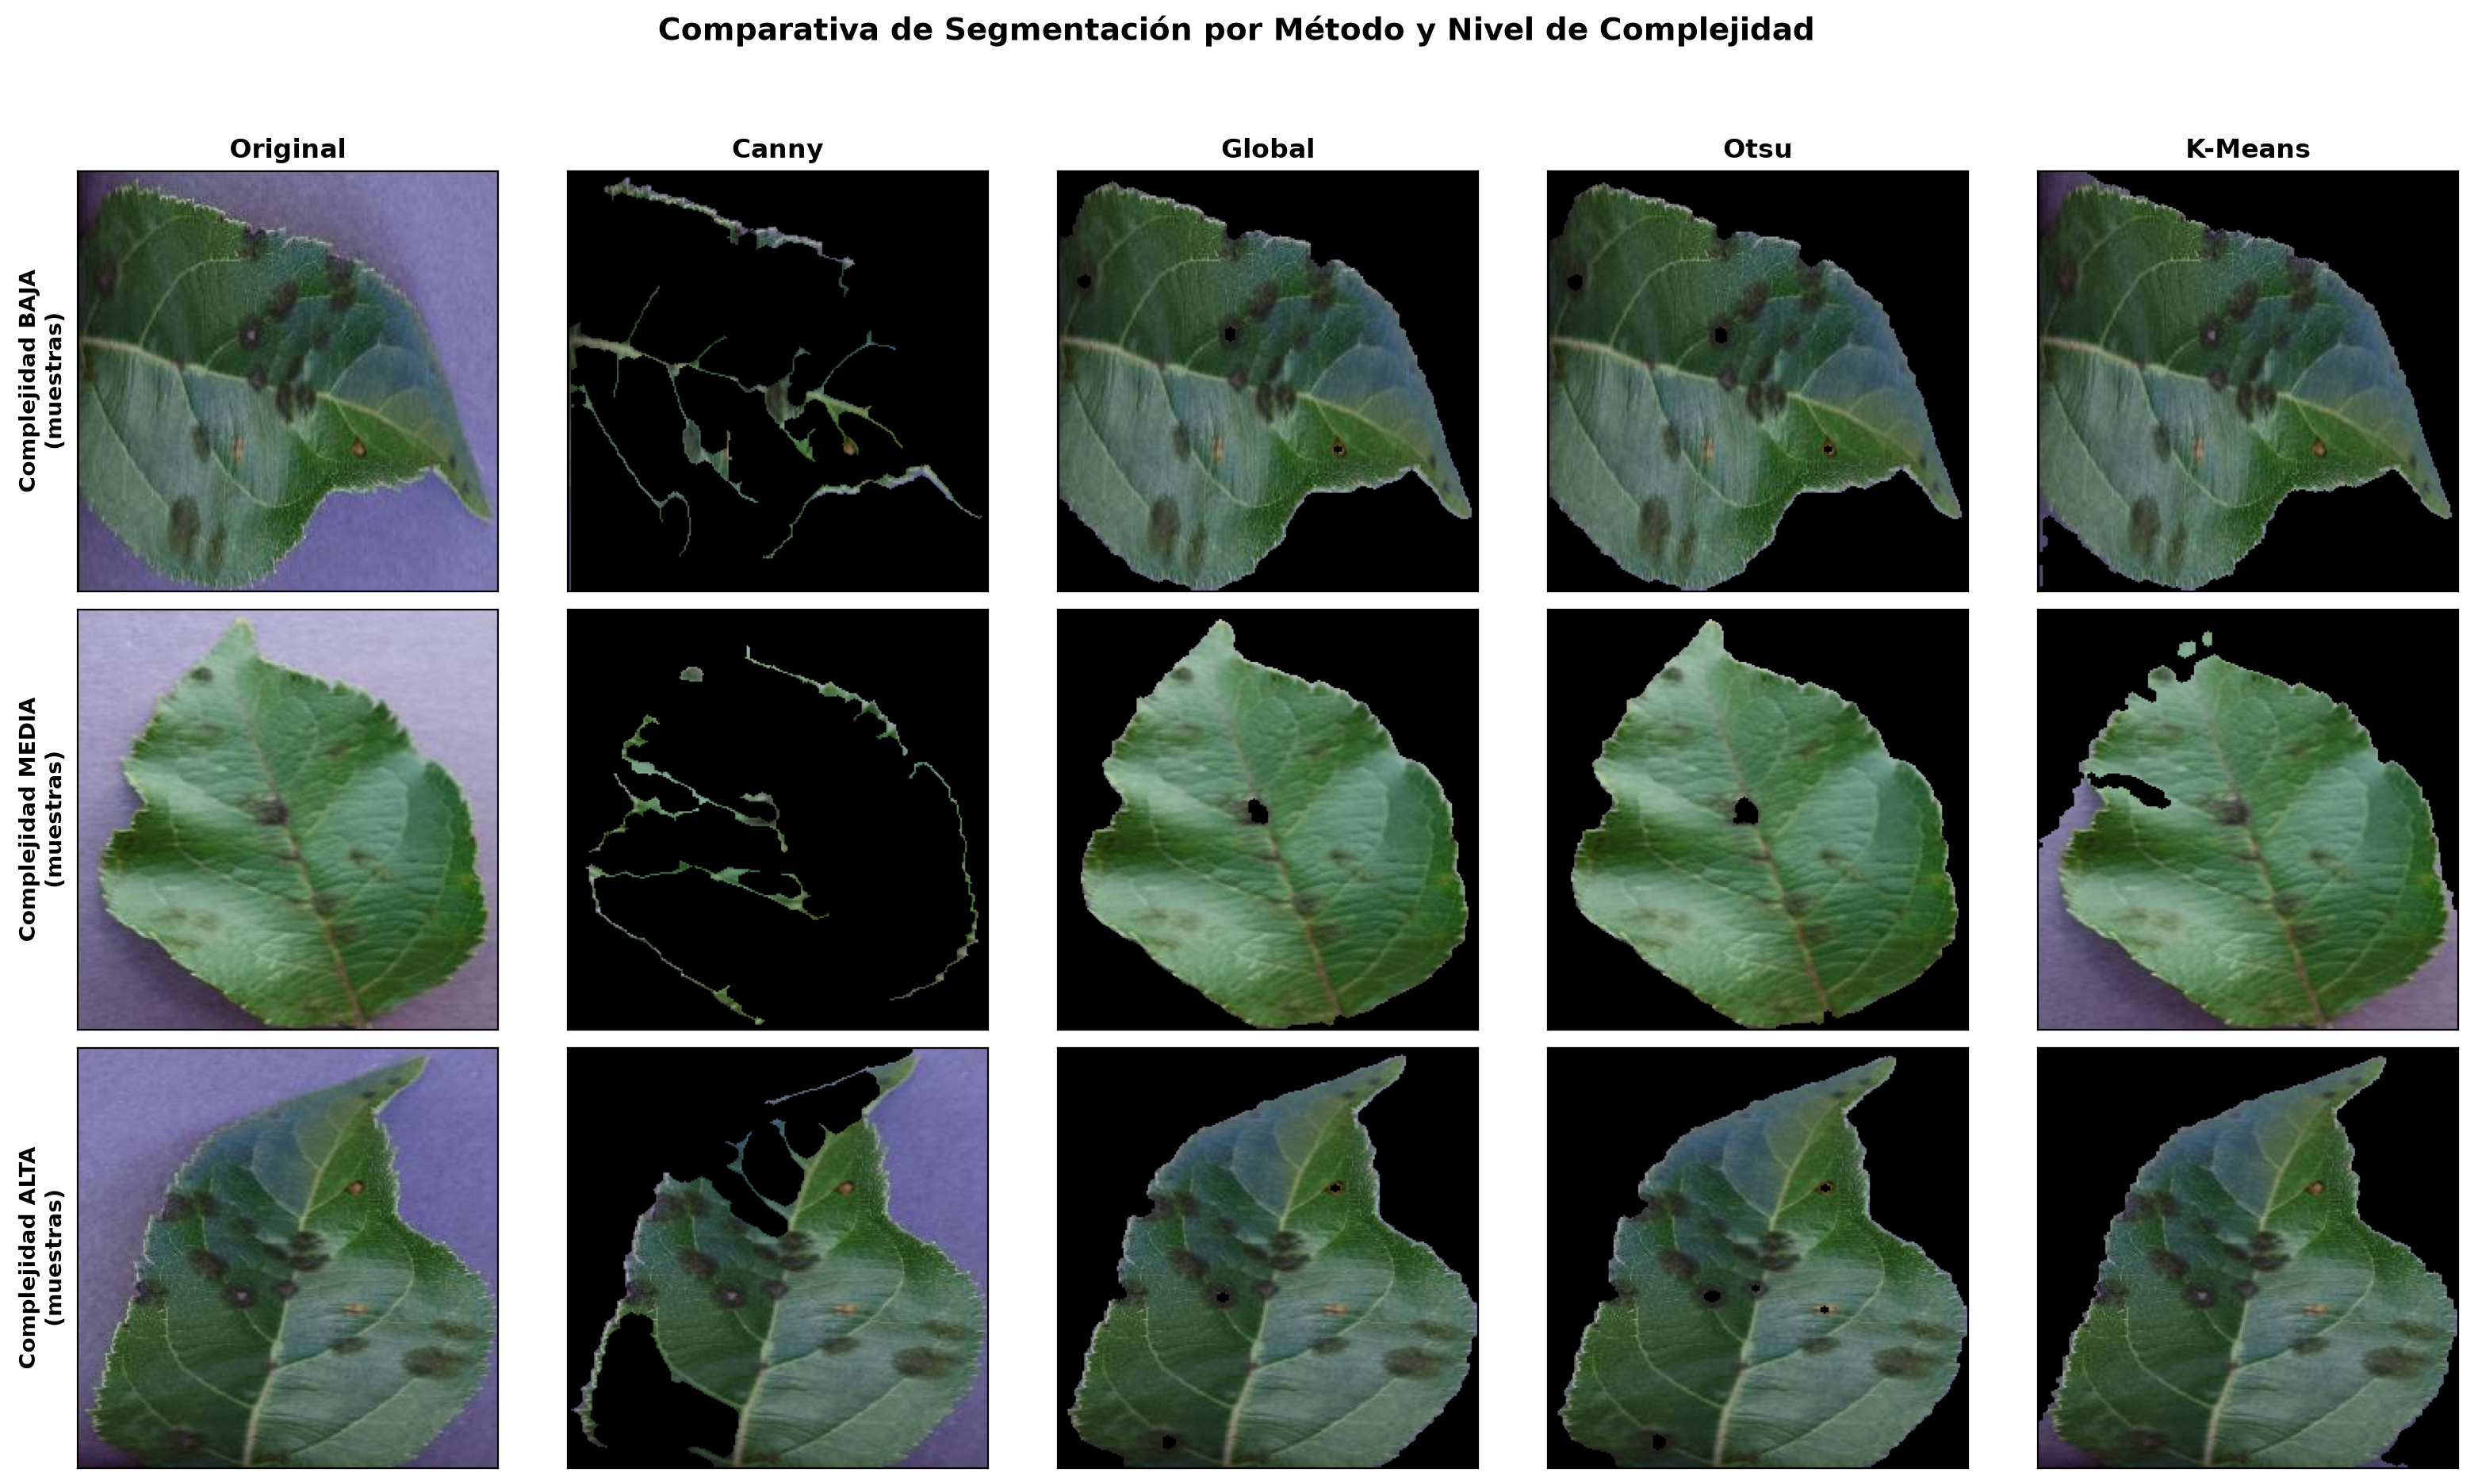
\includegraphics[width=0.92\textwidth]{comparaciones/comparativa_global.png}
\end{frame}

% Conclusiones
\begin{frame}{Discusión y Conclusiones}
    \begin{itemize}
        \item \textbf{Canny:} Produce la mayor definición perimetral foliar, ideal para análisis de área foliar tras el cierre morfológico de contornos.
        \item \textbf{Global vs Otsu:} Otsu supera al umbral global en robustez, al no requerir suposiciones heurísticas y adaptarse a la asimetría de clases.
        \item \textbf{K-Means en $L^*a^*b^*$:} Resultó ser la técnica más precisa frente a sombras y fondos con textura, ya que desacopla la luminancia de las coordenadas cromáticas de clorofila.
        \item \textbf{Perspectiva Fase 3 (Detección de Plagas):} La segmentación multiclase de K-Means ($K=3$) separa con éxito el fondo, el tejido sano y las lesiones de la enfermedad.
    \end{itemize}
\end{frame}

% =============================================================
\section{Referencias}
% =============================================================
\begin{frame}{4. Referencias Bibliográficas}
    \footnotesize
    \begin{enumerate}
        \item Gonzalez, R. C., \& Woods, R. E. (2018). \textit{Digital Image Processing} (4th ed.). Pearson.
        \item Canny, J. (1986). A computational approach to edge detection. \textit{IEEE TPAMI}, (6), 679-698.
        \item Otsu, N. (1979). A threshold selection method from gray-level histograms. \textit{IEEE SMC}, 9(1), 62-66.
        \item MacQueen, J. (1967). Some methods for classification and analysis of multivariate observations. \textit{Proc. 5th Berkeley Symp. Math. Statist. Prob.}, 1(14), 281-297.
        \item Szeliski, R. (2022). \textit{Computer Vision: Algorithms and Applications} (2nd ed.). Springer.
        \item OpenCV Development Team. (2026). \textit{OpenCV Documentation: Image Processing}. \url{https://docs.opencv.org}
        \item Kaggle / Vipul Gaurav. (2019). \textit{New Plant Diseases Dataset (Augmented)}. \url{https://www.kaggle.com/datasets/vipoooool/new-plant-diseases-dataset}
        \item Barbedo, J. G. A. (2016). A review on the main challenges in automatic plant disease identification. \textit{Biosystems Engineering}, 144, 52-60.
    \end{enumerate}
\end{frame}

\end{document}
